\begin{figure}[ht]
  \centering
  \tikzstyle{vertex}=[draw]
  \tikzstyle{arrow}=[thick, -latex]

  \begin{subfigure}[b]{0.3\textwidth}
    \centering
    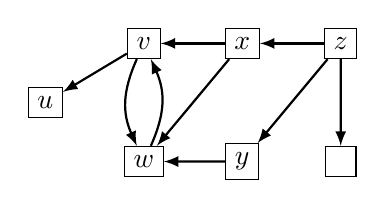
\begin{tikzpicture}[xscale=1.25, yscale=0.75]
      \node[vertex] (u) at (0, 0) {$u$};
      \node[vertex] (v) at (1, 1) {$v$};
      \node[vertex] (w) at (1, -1) {$w$};
      \node[vertex] (x) at (2, 1) {$x$};
      \node[vertex] (y) at (2, -1) {$y$};
      \node[vertex] (z) at (3, 1) {$z$};
      \node[vertex] (unknown) at (3, -1) {\phantom{z}};

      \draw[arrow] (v) to (u);
      \draw[arrow, bend right=15] (v) to (w);
      \draw[arrow, bend right=15] (w) to (v);
      \draw[arrow] (x) to (v);
      \draw[arrow] (x) to (w);
      \draw[arrow] (y) to (w);
      \draw[arrow] (z) to (x);
      \draw[arrow] (z) to (y);
      \draw[arrow] (z) to (unknown);
    \end{tikzpicture}
    \caption{A partial instance graph}\figlabel{PartialInstanceGraph}
  \end{subfigure}
  %
  \begin{subfigure}[b]{0.3\textwidth}
    \centering
    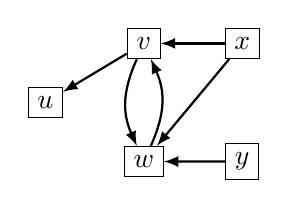
\begin{tikzpicture}[xscale=1.25, yscale=0.75]
      \node[vertex] (u) at (0, 0) {$u$};
      \node[vertex] (v) at (1, 1) {$v$};
      \node[vertex] (w) at (1, -1) {$w$};
      \node[vertex] (x) at (2, 1) {$x$};
      \node[vertex] (y) at (2, -1) {$y$};

      \draw[arrow] (v) to (u);
      \draw[arrow, bend right=15] (v) to (w);
      \draw[arrow, bend right=15] (w) to (v);
      \draw[arrow] (x) to (v);
      \draw[arrow] (x) to (w);
      \draw[arrow] (y) to (w);
    \end{tikzpicture}
    \caption{The eligibile suffix}\figlabel{EligibleSuffix}
  \end{subfigure}
  %
  \begin{subfigure}[b]{0.3\textwidth}
    \centering
    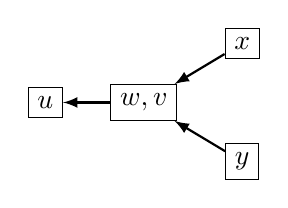
\begin{tikzpicture}[xscale=1.25, yscale=0.75]
      \node[vertex] (u) at (0, 0) {$u$};
      \node[vertex] (vw) at (1, 0) {$w,v$};
      \node[vertex] (x) at (2, 1) {$x$};
      \node[vertex] (y) at (2, -1) {$y$};

      \draw[arrow] (vw) to (u);
      \draw[arrow] (x) to (vw);
      \draw[arrow] (y) to (vw);
    \end{tikzpicture}
    \caption{The condensation}\figlabel{Condensation}
  \end{subfigure}

  \caption{}\figlabel{ExampleConflictGraph}
\end{figure}
